\documentclass[a4paper,10pt]{article}
\usepackage{amsthm}
\usepackage[language = auto, style = numeric, backend = biber, abbreviate = false, dateabbrev = long, alldates = long]{biblatex}
\usepackage{booktabs}
\usepackage[margin=1.3in]{geometry}
\usepackage{graphicx}
\usepackage{minted}
\usepackage{pgfplots}
\usepackage{subfig}
\usepackage{tabulary}
\usepackage{tikz}
\usepackage{todonotes}
\usepackage{xcolor}

\DeclareFieldFormat[software,manual]{title}{#1}
\addbibresource{bibliography.bib}

\usepackage[T1]{fontenc}
\usepackage[charter]{mathdesign}
\usepackage[scaled]{beramono,berasans}
\usepackage{microtype}

\usepackage[bookmarks, colorlinks, linkcolor = ugentblue, citecolor=ugentblue, urlcolor=ugentblue, pdftitle={A beamer presentation class theme for the University of Ghent}, pdfauthor={Pieter Belmans}]{hyperref}

\usemintedstyle{ugent}

\theoremstyle{definition}
\newtheorem{note}{Note}
\newlength\figurewidth
\newlength\figureheight

\title{A \texttt{beamer} presentation class theme for the University of Ghent}
\author{Pieter Belmans\thanks{e-mail: \href{mailto:pieter.belmans@ugent.be}{\nolinkurl{pieter.belmans@ugent.be}}, personal website \url{http://pbelmans.wordpress.com}}}
\date{Version 1.3 \\ \today}

% Pantone 534: global
\definecolor{ugentblue}{RGB}{10,30,96}
% Pantone 130: generic colour
\definecolor{ugentyellow}{RGB}{255,179,0}


% Pantone 103c: Faculty of Literature & Philosophy
\definecolor{ugent-lw}{RGB}{198,173,15}
% Pantone 485c: Faculty of Law
\definecolor{ugent-re}{RGB}{204,12,0}
\definecolor{ugent-re2}{RGB}{216,30,0} % not the actual 485, but looks closer
% Pantone 292c: Faculty of Science
\definecolor{ugent-we}{RGB}{117,178,221}
% Pantone 702: Faculty of Medicine and Health Sciences
\definecolor{ugent-ge}{RGB}{214,96,109}
% Pantone 272c: Faculty of Engineering and Architecture
\definecolor{ugent-tw}{RGB}{94,104,196} % but there are other options
% Pantone 556c: Faculty of Economics and Business Administration
\definecolor{ugent-eb}{RGB}{122,168,145}
% Pantone 2583c: Faculty of Veterinary Medicine
\definecolor{ugent-di}{RGB}{148,79,165}
% Pantone 1655c: Faculty of Psychology and Educational Sciences
\definecolor{ugent-pp}{RGB}{249,86,2}
% Pantone 3262c: Faculty of Bioscience Engineering
\definecolor{ugent-la}{RGB}{0,193,181}
% Pantone purple: Faculty of Pharmaceutical Sciences
\definecolor{ugent-fw}{RGB}{165,68,153}
% Pantone 375c: Faculty of Political and Social Sciences
\definecolor{ugent-ps}{RGB}{140,214,0}


\newcommand\colorsquare[2]{\colorbox{#2}{\rule{0mm}{#1}\rule{#1}{0mm}}}
\newcommand\colorsquareseries[2]{%
  \colorsquare{#1}{#2}%
  \colorsquare{#1}{#2!75!white}%
  \colorsquare{#1}{#2!50!white}%
  \colorsquare{#1}{#2!15!white}%
  \colorsquare{#1}{#2!10!white}%
  \colorsquare{#1}{#2!5!white}%
}

\begin{document}

\maketitle

\begin{abstract}
  This is a theme for the \LaTeX\ \texttt{beamer} class for presentations. It has been designed to match the official UGent templates for Microsoft PowerPoint\textsuperscript{\textregistered} while doing away with some of the shortcomings of it within the \texttt{beamer} framework. If you would like to give a scientific presentation with all the benefits you get from using \LaTeX, this theme is for you.\footnote{Note that there exists another \texttt{beamer} theme for the University of Ghent (or at least the Faculty of Engineering and Architecture) designed by \textsc{Harald Devos} \cite{devos-theme}. In contrast to this theme, it is not designed with compliance to the official themes in mind and it is not tailored to easy integration with the different faculties.}

  It is an adaption of Nico Schl\"omers \texttt{ua-beamer} \cite{ua-beamer}. The philosophy of the theme, its documentation and especially everything related to colors is heavily based on his work.
\end{abstract}


\section{Installation}

\subsection{Requirements}
  The theme is an addendum for the \LaTeX\ \texttt{beamer} class, hence it is assumed that you have a running \LaTeX{} installation together with the \texttt{beamer} package \cite{beamer-repository} and its dependencies. If not already the case, it will also certainly be a good idea to make yourself familiar with the \texttt{beamer} class. The excellent manual \cite{beamer-manual} will serve you well.

\subsection{Getting the package}

The package is distributed via GitHub \cite{ugent-beamer}. You can get the latest releases there, as well as additional information about the package. More specifically the Downloads page located at \url{https://github.com/pbelmans/ugent-beamer/downloads} will serve most of your needs. If you would like to stay on the bleeding edge of development, you can get access to the Git repository by
\begin{minted}[frame=lines]{sh}
$ git clone git@github.com:pbelmans/ugent-beamer.git
\end{minted}
You are free to improve and extend the implementation, preferably by forking and merging to keep development centralized.


\subsection{First run}
Once you have the files, all that is required for the theme to work is putting the files into a directory where \LaTeX{} can find them. This boils down to mimicking the so called TDS (or \TeX\ Directory Structure).

In case you're using your favorite flavor of Unix (and/or \TeX Live) you need to have a local directory (this will probably be \verb|~/texmf/|) and you need to place all the files from the \verb|theme/| folder in the directory \verb|~/texmf/tex/latex/beamer/themes/UGent/|, finishing it by running \verb|texhash|.

If on the other hand you're on Windows (and I assume you are using MiK\TeX, as does 100\% of the population based on my experience) the walkthrough at \url{http://docs.miktex.org/manual/localadditions.html} explains thoroughly and with \emph{many} pictures how to create a local installation. If you've done this you have to put the files from \verb|theme/| in the newly created directory structure as explained in the case of a Unix install, i.e.\ if you've followed the tutorial to the letter the files will be placed in \verb|C:\Local TeX Files\tex\latex\beamer\themes\UGent\| and don't forget to Refresh FNDB as explained at \url{http://docs.miktex.org/manual/configuring.html#fndbupdate}. You might not care about nice installs in which case you can just put everything in \verb|C:\Program Files\MiKTeX 2.9\tex\latex\beamer\themes\UGent\| but you'll need administrator privileges.

\begin{figure}[t]
  \centering
  \setlength{\figurewidth}{6cm}
  \subfloat[][The first two pages, no faculty specified.]{%
    \label{subfigure:example-output-normal-a}
    \frame{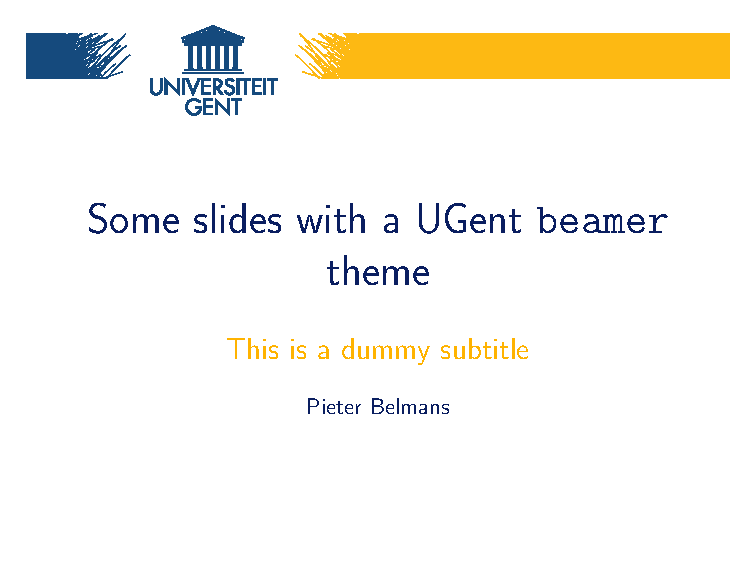
\includegraphics[width=\figurewidth]{figures/slide-1}}%
    \qquad
    \frame{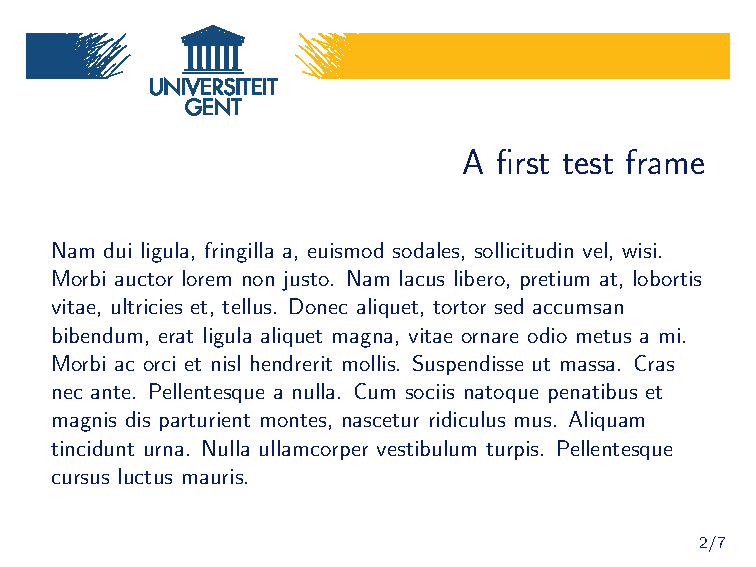
\includegraphics[width=\figurewidth]{figures/slide-2}}%
  }

  \subfloat[][The first two pages, with \texttt{faculty=lw} and \texttt{language=english} specified.]{%
    \label{subfigure:example-output-normal-b}
    \frame{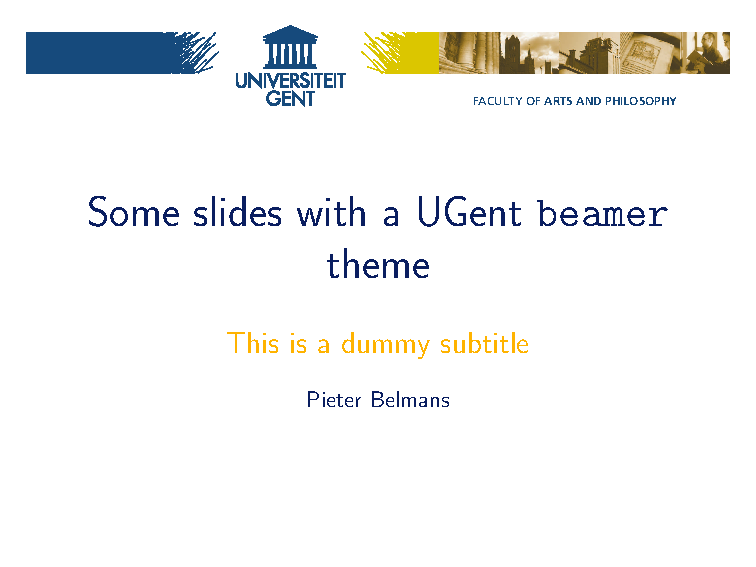
\includegraphics[width=\figurewidth]{figures/slide-faculty-1}}%
    \qquad
    \frame{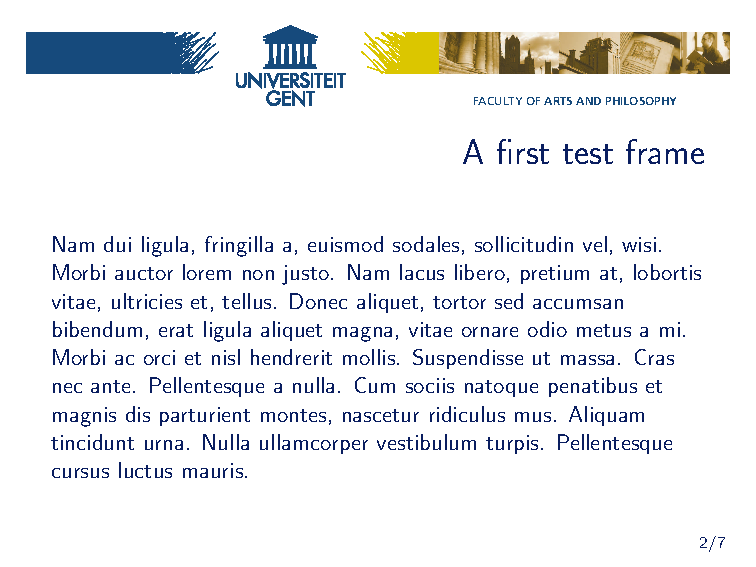
\includegraphics[width=\figurewidth]{figures/slide-faculty-2}}%
  }
  \caption{The first two slides in two different configurations of the UGent \texttt{beamer} theme}
  \label{figure:example-output}
\end{figure}

If everything seems okay, you can check whether you can actually produce a presentation with the UGent theme by either creating a minimal test file (see Listing \ref{listing:minimal-example}) or by compiling the \LaTeX-document provided in the \verb!example/! folder of this package. If you've decided to build the example file, you should get the output as given in Figure~\ref{figure:example-output}\subref{subfigure:example-output-normal-a}, but with the appropriate date.

\begin{note}
  You might need to install more \LaTeX{} packages when running the provided example file (e.g., the \texttt{lipsum} package).
\end{note}

\begin{note}
  If you wish to remove the date from the slides, add \mint{tex}|\date{}|. To control the language in which the date is printed (if you opt for automatic dates), use the \texttt{babel} package \cite{babel}. You will probably need to add \mint{tex}|\usepackage[dutch]{babel}| to your preamble. Remark that this is independent of the \texttt{language=} option as explained in Table~\ref{table:options}.
\end{note}

\begin{listing}[ht]
  \inputminted[frame=lines]{latex}{minimal.tex}
  \caption{A minimalistic test file for the UGent \texttt{beamer} theme.}
  \label{listing:minimal-example}
\end{listing}


\section{Theme options}

The theme comes with several options, all of which can be given in a comma-separated list:
\begin{minted}[frame=lines]{tex}
\usetheme[options]{UniversiteitGent}
\end{minted}
The complete list of options that are currently supported is given in Table~\ref{table:options}.

\begin{table}
  \begin{tabulary}{12cm}{p{3cm}L}
    \toprule
    \texttt{faculty=} & Every faculty can (or should) use its own header, as explained at \url{http://www.ugent.be/nl/werken/organisatie/huisstijl/kantoor/presentaties.htm} (only available to UGent members). This option needs a value, see Table~\ref{table:faculty-values} for an overview. Providing this value will only change the header, but it is related to the options \texttt{language} and \texttt{usecolours}. \\\midrule
    \texttt{language=} & The official template provides both an English and a Dutch header for each faculty, the default is taken to be the \emph{Dutch version}. In case you want to use the English version, provide the option \texttt{language=english}. Remark that the default corresponds to \texttt{language=dutch}, but it is not necessary to provide this. This valued approach is written with future extension in mind. \\\midrule
    %\texttt{nophotos} & If you have provided a value for \texttt{faculty=} and specify this option the pictures in the frame header will be replaced by a monochromous header with the correct faculty color. \\\midrule
    \texttt{footline} \par \texttt{footline=} & Place information about the presentation in the footline. Currently this means that the author is typeset in the center, and the default is to place the institute (as provided by the \verb|\institute| macro available in \textsc{Beamer}) in the left. It is possible to pass a parameter, the only available value is \texttt{sections} in which case the current section (if any) is printed. This serves as an alternative to the navigation bar in some themes, which is ugly. All other values (including no value) are considered as the default. \\\midrule
    \texttt{usecolors} & If you have provided a value for \texttt{faculty=} and specify this option the faculty color (which is featured in the header) will be used in other parts of the presentation, e.g.\ in an \texttt{alertblock}. Otherwise the standard color \texttt{ugentyellow} is used (see Section~\ref{section:colors}). \\\midrule
    \texttt{framenumber} & The \texttt{framenumber} option makes sure that the number of the current frame is displayed. \\\midrule
    \texttt{totalframenumber} & With \texttt{framenumber} turned on, the \texttt{totalframenumber} option makes sure that the total number of frames is displayed alongside with the current frame number.\\\bottomrule
  \end{tabulary}
  \caption{All possible options of the UGent \texttt{beamer} theme}
  \label{table:options}
\end{table}

\begin{note}
  Currently the \texttt{beamer} option \verb|compress| is not supported. The idea of the UA \texttt{beamer} theme of using less vertical margin is a good idea, but it is not feasible in the context of a theme that relies on a header (instead of a logo). In a way this option is always set, because I have disabled the navigation bar regardless of any options.
\end{note}

\begin{note}
  Specifying a wrong value for the \verb|language=| option, or using \verb|usecolors| without specifying a value for \verb|faculty=| will result in errors.
\end{note}


\section{Colors}
\label{section:colors}

\subsection{Background on the official colors}
If you don't care about the technical details, you can skip this and directly go to Subsection \ref{subsection:usingthecolors}.

\vspace{1em}

The two official colors of the UGent, a blue and a yellow tone, are originally given in PMS format, a \emph{proprietary} format issued by the Pantone Inc.\ corporation. One particular feature of the PMS color format is that it is, as opposed to RGB or CMYK, \emph{device independent}. This means that the definition of the color does not consist of instructions such as \enquote{put 37\% red, 12\% green, and 45\% blue and mix it all together}, but really is a concise description of what the final result, be it printed or displayed, physically looks like on the medium under determined ambient light conditions.

The PMS format is richer than RGB in the sense that it can embrace fluorescence effects, gold or silver shine, special coatings (matte and brilliant), in general everything that has to do with the actual appearance of the color on the medium. It comes thus as no surprise that there is no (exact) mapping between the PMS and RGB color spaces; more specifically: the mapping -- if it exists -- is device-dependent.

The \emph{only} way to get a perfect PMS 534 blue, for example, is to have a the plot file ready with the (proprietary) PMS color information in it, and have it printed on a PMS-ready printer which needs to be filled the special PMS 534 ink beforehand. This process is eponymous for colors which are not composed of different types of (yellow, blue, red) inks: they are called \emph{single-spot colors}, and most Pantone\textsuperscript{\textregistered} colors are of such kind.


\subsection{Conversion to RGB/CMYK}

When the computer screen or any other non-PMS-ready medium is the primary output source, having such rigorous rules may be rather obstructive. To overcome such restrictions, many vendors of graphical software try to translate PMS into RGB/CMYK by making use of special monitor color calibration data (e.g., the ICC color profiles, \verb!.icc!). Unfortunately, if files containing PMS color information are displayed (printed) with programs (printers) which do not support PMS mechanisms (which is most often the case in non-professional environments), the color output will look disturbed. On top of that, and surprisingly for the novice, the output will look disturbed in different ways on different screens (printers) because of the inherent device-dependence of PMS.

That is why this theme aims to use non-PMS versions of the UGent's official colors, where I have taken the RGB values used in specifying the colors used in the theme by color picking the resulting \verb|pdf|'s of the headers. That way regardless of whether they use the correct colors everything is consistent.

Now, as explained above there is no device-independent conversion between the original PMS directives and the CMYK color space; several tables exist which are valid for different work environments. On the official sites of the UGent (see \url{http://www.ugent.be/nl/werken/organisatie/huisstijl/elementen/loc_index#kleuren}) you'll find particular RGB values for \verb|ugentblue| and \verb|ugentyellow| while lacking values for the faculty colors. Other resources, e.g., \cite{conversion-chart}, provide other numbers (see Table \ref{table:blues-and-yellows}).

\newlength\boxsize
\setlength\boxsize{2cm}
\begin{table}
  \centering
  \begin{tabular}{cccc}
    \definecolor{ugentbluergb}{RGB}{10,30,96}\colorbox{ugentbluergb}{\rule{0mm}{\boxsize}\rule{\boxsize}{0mm}}
    & \definecolor{ugentbluecmyk}{cmyk}{0.8726,0.6981,0.2617,0.0436}\colorbox{ugentbluecmyk}{\rule{0mm}{\boxsize}\rule{\boxsize}{0mm}}
    & \colorbox{ugentblue}{\rule{0mm}{\boxsize}\rule{\boxsize}{0mm}} \\[2mm]
    \definecolor{ugentyellowrgb}{RGB}{255,179,0}\colorbox{ugentyellowrgb}{\rule{0mm}{\boxsize}\rule{\boxsize}{0mm}}
    & \definecolor{ugentyellowcmyk}{cmyk}{0,0.2617,0.8726,0}\colorbox{ugentyellowcmyk}{\rule{0mm}{\boxsize}\rule{\boxsize}{0mm}}
    & \colorbox{ugentyellow}{\rule{0mm}{\boxsize}\rule{\boxsize}{0mm}} \\[2mm]
  \end{tabular}
  \caption{PMS 534 and PMS 130 translated to CMYK/RGB in different ways. Left to right: UGent website \cite{ugent-color-guide} RGB, UGent website \cite{ugent-color-guide} CMYK, actual value in use by the theme as determined by color picking the headers. To determine which version is closest to the actual colors PMS 534 and PMS 130 on your monitor/printer/beamer, you would need a physical color sample (such as provided on the Pantone\textsuperscript{\textregistered} charts) to compare.}
  \label{table:blues-and-yellows}
\end{table}

\subsection{Using the colors}\label{subsection:usingthecolors}


\newlength\facultieswidth
\setlength\facultieswidth{8cm}
\newlength\colorwidth
\setlength\colorwidth{2.75cm}
\setlength\figurewidth{5mm}
\begin{table}
  \centering
  \small
  \begin{tabular}{cp{\facultieswidth}p{\colorwidth}c}
    \toprule
    value & faculty & color & example \\\midrule
    \verb|lw|
    & \parbox\facultieswidth{Faculty of Literature and Philosophy \\ Faculteit Letteren en Wijsbegeerte}
    & \parbox\colorwidth{Pantone 103c \\ \extractcolorspecs{ugent-lw}\modelspec\colorspec \convertcolorspec\modelspec\colorspec{RGB}\colorspec RGB\ \colorspec}
    & \colorsquare\figurewidth{ugent-lw} \\
    \verb|re|
    & \parbox\facultieswidth{Faculty of Law \\ Faculteit Rechtsgeleerdheid}
    & \parbox\colorwidth{Pantone 485c \\ \extractcolorspecs{ugent-re}\modelspec\colorspec \convertcolorspec\modelspec\colorspec{RGB}\colorspec RGB\ \colorspec}
    & \colorsquare\figurewidth{ugent-re} \\
    \verb|we|
    & \parbox\facultieswidth{Faculty of Science \\ Faculteit Wetenschappen}
    & \parbox\colorwidth{Pantone 292c \\ \extractcolorspecs{ugent-we}\modelspec\colorspec \convertcolorspec\modelspec\colorspec{RGB}\colorspec RGB\ \colorspec}
    & \colorsquare\figurewidth{ugent-we} \\
    \verb|ge|
    & \parbox\facultieswidth{Faculty of Medicine and Health Sciences \\ Faculteit Geneeskunde en Gezondheidswetenschappen}
    & \parbox\colorwidth{Pantone 702 \\ \extractcolorspecs{ugent-ge}\modelspec\colorspec \convertcolorspec\modelspec\colorspec{RGB}\colorspec RGB\ \colorspec}
    & \colorsquare\figurewidth{ugent-ge} \\
    \verb|tw|
    & \parbox\facultieswidth{Faculty of Engineering and Architecture \\ Faculteit Ingenieurswetenschappen en Architectuur}
    & \parbox\colorwidth{Pantone 272c \\ \extractcolorspecs{ugent-tw}\modelspec\colorspec \convertcolorspec\modelspec\colorspec{RGB}\colorspec RGB\ \colorspec}
    & \colorsquare\figurewidth{ugent-tw} \\
    \verb|eb|
    & \parbox\facultieswidth{Faculty of Economcs and Business Administration \\ Faculteit Economie en Bedrijfskunde}
    & \parbox\colorwidth{Pantone 556c \\ \extractcolorspecs{ugent-eb}\modelspec\colorspec \convertcolorspec\modelspec\colorspec{RGB}\colorspec RGB\ \colorspec}
    & \colorsquare\figurewidth{ugent-eb} \\
    \verb|di|
    & \parbox\facultieswidth{Faculty of Veterinary Medicine \\ Faculteit Diergeneeskunde}
    & \parbox\colorwidth{Pantone 2583c \\ \extractcolorspecs{ugent-di}\modelspec\colorspec \convertcolorspec\modelspec\colorspec{RGB}\colorspec RGB\ \colorspec}
    & \colorsquare\figurewidth{ugent-di} \\
    \verb|pp|
    & \parbox\facultieswidth{Faculty of Psychology and Educational Sciences \\ Faculteit Psychologie en Pedagogische Wetenschappen}
    & \parbox\colorwidth{Pantone 1655c \\ \extractcolorspecs{ugent-pp}\modelspec\colorspec \convertcolorspec\modelspec\colorspec{RGB}\colorspec RGB\ \colorspec}
    & \colorsquare\figurewidth{ugent-pp} \\
    \verb|la|
    & \parbox\facultieswidth{Faculty of Bioscience Engineering \\ Faculteit Bio-ingenieurswetenschappen}
    & \parbox\colorwidth{Pantone 3262c \\ \extractcolorspecs{ugent-la}\modelspec\colorspec \convertcolorspec\modelspec\colorspec{RGB}\colorspec RGB\ \colorspec}
    & \colorsquare\figurewidth{ugent-la} \\
    \verb|fw|
    & \parbox\facultieswidth{Faculty of Pharmaceutical Sciences \\ Faculteit Farmaceutische Wetenschappen}
    & \parbox\colorwidth{Pantone purple \\ \extractcolorspecs{ugent-fw}\modelspec\colorspec \convertcolorspec\modelspec\colorspec{RGB}\colorspec RGB\ \colorspec}
    & \colorsquare\figurewidth{ugent-fw} \\
    \verb|ps|
    & \parbox\facultieswidth{Faculty of Political and Social Sciences \\ Faculteit Politieke en Sociale Wetenschappen}
    & \parbox\colorwidth{Pantone 375c \\ \extractcolorspecs{ugent-ps}\modelspec\colorspec \convertcolorspec\modelspec\colorspec{RGB}\colorspec RGB\ \colorspec}
    & \colorsquare\figurewidth{ugent-ps} \\\bottomrule
  \end{tabular}
  \caption{Overview of the faculties and their respective colors}
  \label{table:faculty-values}
\end{table}

Getting a consistent look-and-feel throughout your presentations requires sticking to a particular style scheme, most of which is being implemented in the \texttt{beamer} style file already. One particular aspect, though, can only be controlled by the user, and that is the colors that are used in the running text, tables, and figures.

Although essentially consistent of only two colors, within \texttt{beamer} referred to as \verb!ugentblue! and \verb!ugentyellow! (see Table~\ref{table:all-colors}, provide more diversity than one might expect and should be \emph{exclusively} used in all the slides. The user should be aware that this directive includes \emph{tables, figures, and graphics of most kinds}. For an example of this behavior see Figure \ref{figure:colored-graphs}.

\setlength\figurewidth{10cm}
\setlength\figureheight{5cm}
\begin{figure}[ht]
  \centering
  \begin{tikzpicture}

% Axis at [0.13 0.11 0.78 0.81]
\begin{axis}[
axis on top,
scale only axis,
width=\figurewidth,
height=\figureheight,
xmin=0, xmax=10,
ymin=0, ymax=7
]

\addplot [
color=ugentblue,
solid,
line width=1pt
] coordinates{
 (0,5.23398) (1,4.38268) (2,4.69238) (3,4.32081) (4,3.54144) (5,3.72536) (6,3.16156) (7,2.59604) (8,2.20231) (9,2.60195) (10,1.60575)
};

\addplot [
color=ugentyellow,
solid,
line width=1pt
] coordinates{
 (0,2.02709) (1,2.02644) (2,1.68711) (3,1.84761) (4,1.78782) (5,1.24044) (6,1.26026) (7,0.992143) (8,0.859557) (9,0.689706) (10,0.36891)
};

\addplot [
color=ugentblue!50!white,
solid,
line width=1pt
] coordinates{
 (0,3.2703) (1,3.30947) (2,3.74723) (3,3.45218) (4,3.3806) (5,3.13813) (6,2.81847) (7,2.79316) (8,2.64385) (9,3.01041) (10,2.72024)
};

\addplot [
color=ugentyellow!50!white,
solid,
line width=1pt
] coordinates{
 (0,5.49163) (1,4.97712) (2,5.031) (3,5.42669) (4,5.41402) (5,5.4996) (6,5.311) (7,5.34227) (8,5.46331) (9,5.46677) (10,5.12875)
};

\addplot [
color=ugentblue!25!white,
solid,
line width=1pt
] coordinates{
 (0,5.56199) (1,5.2627) (2,5.27883) (3,5.38474) (4,5.90686) (5,6.11345) (6,6.04402) (7,6.36515) (8,6.62563) (9,6.38024) (10,6.33876)
};

\addplot [
color=ugentyellow!25!white,
solid,
line width=1pt
] coordinates{
 (0,3.7947) (1,4.08811) (2,4.28361) (3,4.45264) (4,4.46625) (5,5.28088) (6,5.32715) (7,5.54452) (8,5.439) (9,5.99242) (10,6.35941)
};

\addplot [
color=ugent-re,
solid,
line width=1pt
] coordinates{
 (0,1.43939) (1,1.51392) (2,2.30537) (3,2.05355) (4,3.05479) (5,2.9632) (6,3.16279) (7,3.3234) (8,4.15725) (9,4.278) (10,4.78022)
};

\end{axis}

\end{tikzpicture}

  \caption{Example usage of the official colors within a set of graphs, using also an exception color, which happens to be \texttt{ugent-re}.}
  \label{figure:colored-graphs}
\end{figure}

If you need to emphasize a particular aspect in your slides (graphs, tables), you can (within \texttt{beamer}) use the \verb!\alert{}! macro (e.g., \verb!\alert{This is alerted text.}!). For the situation where something needs to stick out in a pie chart, for example, where the ordinary colors (UGent blue and yellow) have been used up already, you can choose to use the color of your faculty (if specified) which is available in \verb|ugent-faculty| or choose a color from Table~\ref{table:faculty-values} as these have been designed to match the standard colors of UGent. A color from this table is accessed by prefixing the code from the table with \verb|ugent-|, i.e.\ to access the Pantone 485c from the Faculty of Law you use \verb|ugent-re|. These are to be used scarcely and strictly for highlighting purposes (see, for example, Figure \ref{figure:colored-graphs}).

As said earlier, the color of your faculty (if specified) is available in the variable \verb|ugent-faculty|. If for some reason you don't like this color and wish to use another, it can be easily reset using
\begin{minted}[frame=lines]{tex}
\colorlet{ugent-faculty}{ugent-we}
\end{minted}
where we have set the color of our faculty to the Pantone 292c as used by the Faculty of Sciences. 

\begin{note}
  If you wish to include highlighted code fragments, it is a good idea to use Pygments \cite{pygments} in conjunction with the \texttt{ugent-pygments-style} \cite{ugent-pygments-style}. This style file uses the official colors as explained in this section, hence it is well-suited for use in this \texttt{beamer} theme.
\end{note}

\begin{table}[ht]
  \setlength\figurewidth{15mm}
  \centering
  \small
  \begin{tabulary}{\textwidth}{LCCC}
    \toprule
    Color sample & \colorsquare{\figurewidth}{ugentblue!100!white} & \colorsquare{\figurewidth}{ugentblue!75!white} & \colorsquare{\figurewidth}{ugentblue!50!white}\\
    CMYK & (100, 30, 0, 62) & (75, 23, 0, 47) & (50, 15, 0, 31)\\
    RGB  & (0, 61, 100)     & (40, 128, 158)  & (96, 166, 191)\\
    \texttt{beamer} name & \texttt{ugentblue!100!white} & \texttt{ugentblue!75!white} & \texttt{ugentblue!50!white} \\[3mm]
    Color sample & \colorsquare{\figurewidth}{ugentblue!25!white} & \colorsquare{\figurewidth}{ugentblue!10!white} & \colorsquare{\figurewidth}{ugentblue!5!white}\\
    CMYK & (25, 8, 0, 16)  & (10, 3, 0, 6)   & (5, 2, 0, 3)\\
    RGB  & (166, 209, 222) & (218, 235, 242) & (235, 245, 247)\\
    \texttt{beamer} name & \texttt{ugentblue!25!white} & \texttt{ugentblue!10!white} & \texttt{ugentblue!5!white} \\\midrule
  
    Color sample & \colorsquare{\figurewidth}{ugentyellow!100!white} & \colorsquare{\figurewidth}{ugentyellow!75!white} & \colorsquare{\figurewidth}{ugentyellow!50!white}\\
    CMYK & (0, 100, 54, 46) & (0, 75, 41, 35) & (0, 50, 27, 23)\\
    RGB  & (161, 0, 64)     & (184, 46, 101)  & (207, 103, 145)\\
    \texttt{beamer} name & \texttt{ugentyellow!100!white} & \texttt{ugentyellow!75!white} & \texttt{ugentyellow!50!white} \\[3mm]
    Color sample & \colorsquare{\figurewidth}{ugentyellow!25!white} & \colorsquare{\figurewidth}{ugentyellow!10!white} & \colorsquare{\figurewidth}{ugentyellow!5!white}\\
    CMYK & (0, 25, 14, 12)  & (0, 10, 5, 5)   & (0, 5, 3, 2)\\
    RGB  & (232, 174, 197) & (245, 220, 230) & (250, 237, 242)\\
    \texttt{beamer} name & \texttt{ugentyellow!25!white} & \texttt{ugentyellow!10!white} & \texttt{ugentyellow!5!white} \\\midrule
  \end{tabulary}

  \caption{Overview of the two main colors used in theme.}
  \label{table:all-colors}
\end{table}

\clearpage
\printbibliography

\end{document}
